% --- chapter
\newcommand{\chapter}[2][]{
	\newcommand{\chapname}{#2}
	\begin{flushleft}
		\begin{minipage}[t]{\linewidth}
			
\includegraphics[height=1cm]{hdht-logo.png}
			\hspace{0pt}	
			\sffamily\bfseries\large Bài  20. Mạch dao động
			\begin{flushleft}
				\huge\bfseries #1
			\end{flushleft}
		\end{minipage}
	\end{flushleft}
	\vspace{1cm}
	\normalfont\normalsize
}
%-----------------------------------------------------
\chapter[Cấu tạo và nguyên tắc của mạch dao động]{Cấu tạo và nguyên tắc của mạch dao động}
\section{Lý thuyết}
	\subsection {Mạch dao động}
\begin{center}
	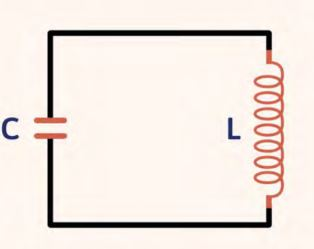
\includegraphics[scale=0.5]{../figs/4-1-1.JPG}
\end{center}
\begin{itemize}
	\item Gồm một tụ điện có điện dung $C$ mắc với một cuộn cảm có độ tự cảm $L$ thành mạch kín.
	\item Nếu điện trở của mạch rất nhỏ, coi như bằng không, thì mạch là một mạch dao động lý tưởng.
\end{itemize}
\subsection{Sự biến thiên điện tích và cường độ dòng điện trong mạch dao động lí tưởng}
Điện tích $q$ của một bản tụ điện và cường độ dòng điện $i$ trong mạch dao động biến thiên điều hòa theo thời gian, $i$ sớm pha $\dfrac{\pi}{2} $ so với $q$.
\begin{equation}
	q=q_0\cos(\omega t +\varphi)\ \text{C}, 
\end{equation}
\begin{equation}
	i=\frac{dq}{dt}=I_0 \cos(\omega +\varphi+ \frac{\pi}{2})\ \text{A},
\end{equation}
trong đó: $I_0=q_0\omega, \omega =\dfrac{1}{\sqrt {LC}}$.
\subsection {Dao động điện từ tự do}
Sự biến thiên điều hòa theo thời gian của điện tích $q$ của một bản tụ điện và cường độ dòng điện $i$ (hoặc cường độ điện trường $\vec{E}$ và cảm ứng từ $\vec{B}$) trong mạch dao động được gọi là dao động điện từ tự do.
\subsection {Chu kì và tần số dao động riêng của mạch dao đông}
Gồm tụ điện có điện dung $C$ mắc với một cuộn cảm có độ tự cảm $L$ thành mạch kín.
\begin{equation}
	T=2\pi \sqrt {LC},
\end{equation}
\begin{equation}
	f=\frac{1}{2\pi\sqrt {LC}},
\end{equation}
trong đó:\\
$L$: Độ tự cảm của cuộn dây ($\text{H}$);\\
$C$: Điện dung của tụ điện ($\text{F}$);\\
$T$: Chu kì dao động ($\text{s}$);\\
$f$: Tần số dao động riêng của mạch dao động ($\text{Hz}$).
\subsection {Năng lượng điện từ}
\begin{itemize}
	\item Tổng năng lượng điện trường trong tụ điện và năng lượng từ trường trong cuộn cảm của mạch gọi là năng lượng điện từ.\\
	\begin{equation}
		W=W_{\text{đ}}+W_{t}=\frac{1}{2}Cu^2+\frac{1}{2}Li^2
	\end{equation}
	\item Nếu không có sự tiêu hao năng lượng thì năng lượng điện từ trong mạch sẽ được bảo toàn.
\end{itemize}
\section{Mục tiêu bài học - Ví dụ minh họa}
\begin{dang}{Xác định chu kỳ, tần số, điện tích của mạch dao động}
	\viduii{2}{
		
		Mạch dao động LC lí tưởng gồm cuộn cảm có độ tự cảm $L = \SI{2}{mH}$ và tụ điện có điện dung $C = \SI{2}{pF}$. Tần số dao động của mạch gần bằng
		\begin{mcq}(4)
			\item $\SI{1}{MHz}$. 
			\item $\SI{2,5}{MHz}$. 
			\item $\SI{1}{kHz}$. 
			\item $\SI{2,5}{kHz}$. 
		\end{mcq}
	}
	{	\begin{center}
			\textbf{Hướng dẫn giải}
		\end{center}
		
		
		Tần số dao động riêng của mạch cho bởi
		
		$$f = \dfrac{1}{2\pi \sqrt{LC}} = \SI{2,5}{MHz}.$$
		
		\textbf{Đáp án: B.}
	
		
		\begin{center}
			\textbf{Câu hỏi tương tự}
		\end{center}
		
	Một mạch dao động gồm một cuộn cảm có độ tự cảm $L = \SI{1}{mH}$ và một tụ điện có điện dung là $C = \SI{0,1}{\mu F}$. Tần số riêng của mạch có giá trị nào?
		
		\textbf{Đáp án:} $f = \text{1,6}\cdot 10^4\ \text{Hz}$.
	}
	\viduii{2}{
		
		Mạch dao động điện từ lí tưởng gồm cuộn dây thuần cảm có độ tự cảm L và tụ điện có điện dung C. Khi tăng điện dung của tụ điện lên 9 lần thì chu kì dao động riêng của mạch
		\begin{mcq}(2)
			\item tăng lên 9 lần. 
			\item tăng lên 3 lần. 
			\item giảm đi 9 lần. 
			\item giảm 3 lần. 
		\end{mcq}
}
{	\begin{center}
		\textbf{Hướng dẫn giải}
	\end{center}
	
	Ban đầu, chu kì dao động riêng của mạch cho bởi công thức 
	
	$$T = 2\pi \sqrt{LC}.$$
	
	Lúc sau, chu kì dao động riêng của mạch cho bởi công thức 
	
	$$T' = 2\pi \sqrt{LC'}.$$ 
	
	Lập tỉ lệ hai biểu thức trên ta được
	
	$$\dfrac{T'}{T} = \sqrt{\dfrac{C'}{C}}.$$
	
	Thay $C' = 9C$ vào biểu thức trên ta được $T' = 3T$.
	
	\textbf{Đáp án: B.}
	
	\begin{center}
		\textbf{Câu hỏi tương tự}
	\end{center}
	
	Mạch dao động điện từ điều hoà gồm cuộn cảm $L$ và tụ điện $C$, khi tăng điện dung của tụ điện lên 4 lần thì chu kỳ dao động của mạch?
	
	\textbf{Đáp án:} tăng lên 2 lần.
}

	
		\viduii{2}{
			Một mạch dao động lí tưởng gồm cuộn cảm thuần có độ tự cảm $\xsi{4}{\mu H}$ và một tụ điện có điện dung biến đổi từ $\xsi{10}{pF}$ đến $\xsi{640}{pF}$. Lấy $\pi^2 = 10$. Chu kì dao động riêng của mạch có giá trị
			\begin{mcq}(2)
				\item từ $\xsi{4,2\cdot10^{-8}}{s}$ đến $\xsi{2,4\cdot10^{-7}}{s}$. 
				\item từ $\xsi{2,24\cdot10^{-8}}{s}$ đến $\xsi{3\cdot10^{-7}}{s}$. 
				\item từ $\xsi{2\cdot10^{-8}}{s}$ đến $\xsi{3,6\cdot10^{-7}}{s}$. 
				\item từ $\xsi{4\cdot10^{-8}}{s}$ đến $\xsi{3,2\cdot10^{-7}}{s}$. 
			\end{mcq}
	}
	{	\begin{center}
			\textbf{Hướng dẫn giải}
		\end{center}
		
		Chu kì dao động riêng trong mạch cho bởi: 
		
		$$T = 2\pi \sqrt{LC}.$$
		
		Khi $C = \xsi{10}{pF}$, ta có:
		
		$$T = 2\pi \sqrt{LC} = \xsi{4\cdot10^{-8}}{s}.$$ 
		
		Khi $C = \xsi{640}{pF}$, ta có:
		
		$$T = 2\pi \sqrt{LC} = \xsi{3,2\cdot10^{-7}}{s}.$$ 
		
		Vậy chu kì dao động riêng của mạch biến thiên từ $\xsi{4\cdot10^{-8}}{s}$ đến $\SI{3,2 e-7}{s}$.
		
		\textbf{Đáp án: D.}
		
		\begin{center}
			\textbf{Câu hỏi tương tự}
		\end{center}
		
			Một mạch dao động lí tưởng gồm tụ điện có điện dung $C$ và cuộn cảm thuần có độ tự cảm $L$, đang thực hiện dao động điện từ tự do với tần số $f$. Nếu tăng điện dung của tụ điện lên 16 lần thì tần số dao động của mạch giảm lượng $\SI{24}{MHz}$. Giá trị của $f$ bằng
		\begin{mcq}(4)
			\item $\SI{48}{MHz}$. 
			\item $\SI{32}{MHz}$. 
			\item $\SI{40}{MHz}$. 
			\item $\SI{36}{MHz}$. 
		\end{mcq}
		
		\textbf{Đáp án: B}.
	}
	\viduii{2}{
		Điện tích của một bản tụ trong mạch dao động $LC$ lí tưởng biến đổi điều hòa có biểu thức là $q = 6\cdot10^{-6} \cos \left( 4000t + \dfrac{\pi}{2} \right)\ \text C$. Tại thời điểm $t = \xsi{10^{-4}}{s}$, điện tích trên bản tụ có độ lớn xấp xỉ bằng 
		\begin{mcq}(2)
			\item $\SI{2,30e-6}{C}$. 
			\item $\SI{5,90e-6}{C}$. 
			\item $\SI{1,15e-6}{C}$. 
			\item $\SI{4,60e-6}{C}$. 
		\end{mcq}
	}
	{	\begin{center}
			\textbf{Hướng dẫn giải}
		\end{center}
	
	Ta thay thời điểm $t = \SI{e-4}{s}$ vào biểu thức điện tích, ta được:
	
	$$ q = \num{6e-6} \cos \left( 4000t + \dfrac{\pi}{2} \right) = -\SI{2,30 e-6}{C}.$$
	
	\textbf{Đáp án: A.}
		
		\begin{center}
			\textbf{Câu hỏi tương tự}
		\end{center}
		
		Điện tích của một bản tụ trong mạch dao động $LC$ đang thực hiện dao động điện từ tự do là $q = 4\cdot10^{-7} \cos \left( 4000t \right)\ \text C$. Điện tích cực đại có độ lớn
		\begin{mcq}(2)
			\item $\xsi{2\sqrt{2}\cdot10^{3}}{C}$. 
			\item $\xsi{22\cdot10^{-7}}{C}$. 
			\item $\xsi{4\cdot10^{-7}}{C}$. 
			\item $\xsi{4\cdot10^{3}}{C}$. 
		\end{mcq}
		
		\textbf{Đáp án: C}.
	}

	\viduii{2}{
		
		Một mạch dao động lí tưởng gồm tụ điện có điện dung $C = 2 \mu \text F$ và cuộn cảm thuần có độ tự cảm $L$, đang thực hiện dao động điện từ tự do. Biết dòng điện qua mạch có dạng $i = 2 \cos \left( 5000t \right)\ \text{mA}$. Giá trị của $L$ bằng
		\begin{mcq}(4)
			\item $\SI{0,05}{H}$. 
			\item $\SI{0,01}{H}$. 
			\item $\SI{0,02}{H}$. 
			\item $\SI{0,04}{H}$. 
		\end{mcq}
	}
	{	\begin{center}
			\textbf{Hướng dẫn giải}
		\end{center}
		
		Tần số dao động riêng của mạch 
		
		$$\omega = \SI{5000}{rad/s}.$$ 
		
		Lại có $\omega = \dfrac{1}{\sqrt{LC}}$ nên suy ra
		 
		$$L = \dfrac{1}{C \omega^2} = \SI{0,02}{H}.$$ 
		
		\textbf{Đáp án: C.}
		
		\begin{center}
			\textbf{Câu hỏi tương tự}
		\end{center}
		
			Điện tích của một bản tụ trong mạch dao động điện từ có phương trình là $q = Q_0 \cos \left( 4\pi \cdot 10^{4}t \right)\ \text C$. Trong đó $t$ tính theo giây. Tần số dao động của mạch là
		\begin{mcq}(2)
			\item $ \SI{1e4}{Hz} $.
			\item $ \SI{20e14}{Hz} $.
			\item $ \SI{2e4}{Hz} $.
			\item $ \SI{2e4}{kHz} $.
		\end{mcq}
		
		\textbf{Đáp án: C}.
	}

\end{dang}

\begin{dang}{Xác định năng lượng điện từ của mạch dao động}
	\viduii{2}{
		
		Một mạch dao động $LC$ có điện trở thuần không đáng kể, tụ điện có điện dung $\SI{5}{\mu \text F}$. Dao động điện từ tự do của mạch $LC$ với hiệu điện thế cực đại ở hai đầu tụ điện bằng $\SI{6}{V}$. Khi hiệu điện thế ở hai đầu tụ điện là $\SI{4}{V}$ thì năng lượng điện từ trong mạch bằng
		\begin{mcq}(4)
			\item $\xsi{9\cdot10^{-5}}{J}$. 
			\item $\xsi{5\cdot10^{-5}}{J}$. 
			\item $\xsi{4\cdot10^{-5}}{J}$. 
			\item $\xsi{10^{-5}}{J}$. 
		\end{mcq}
	}
	{	\begin{center}
			\textbf{Hướng dẫn giải}
		\end{center}
		
			Năng lượng điện từ trong mạch ở thời điểm bất kì cũng chính là năng lượng cực đại của điện trường bên trong tụ điện:
			
		$$W = W_C = \dfrac{1}{2}CU^{2} = \xsi{9\cdot10^{-5}}{J}.$$
		
		\textbf{Đáp án: A.}
		
		\begin{center}
			\textbf{Câu hỏi tương tự}
		\end{center}
			
	Một mạch dao động $LC$ có cuộn thuần cảm có độ tự cảm $L = \SI{0,4}{H}$ và tụ điện có điện dung $C= \SI{40}{\mu F}$ Cường độ dòng điện qua mạch có biểu thức: $i = 2\sqrt 2 \cos 100\pi t\ \text A$. Tính năng lượng dao động của mạch?
	
	\textbf{Đáp án:} $W = \SI{1,6}{J}.$
	}
	\viduii{2}{
	
	Cho một mạch dao động điện từ gồm một tụ điện có điện dung $C = \SI{5}{\mu F}$ và một cuộn thuần cảm có độ tự cảm $L = \SI{50}{mH}$. Biết điện áp cực đại trên tụ là  $\SI{6}{V}$. Tìm năng lượng điện trường và năng lượng từ trường trong mạch khi điện áp trên tụ điện là $\SI{4}{V}$ và cường độ dòng điện $i$ khi đó.
	
}
{	\begin{center}
		\textbf{Hướng dẫn giải}
	\end{center}
	
	Năng lượng điện trường
	
	$$W_\text{đ} = \dfrac{1}{2} Cu^2 = 4 \cdot 10^{-5}\ \text{J}.$$
	
	Năng lượng điện từ
	
	$$W = \dfrac{1}{2}CU_0^2 = 9 \cdot 10^{-5}\ \text J.$$
	
	Cường độ dòng điện $i$
	
	$$ W_\text t =\dfrac{1}{2} Li^2 \Rightarrow i = \SI{0,045}{A}.$$
	
		\begin{center}
		\textbf{Câu hỏi tương tự}
	\end{center}
	
	rong một mạch $LC$, $L = \SI{25}{mH}$ và $C = \SI{1,6}{\mu F}$ ở thời điểm $t = 0$, cường độ dòng điện trong mạch bằng $\SI{6,93}{mA}$, điện tích ở trên tụ điện bằng $\SI{0,8}{\mu C}$. Tính năng lượng của mạch dao động.
	
	\textbf{Đáp án:} $W = \text{0,8}\cdot 10^{-6}\ \text J.$
}

\end{dang}
